\documentclass[aspectratio=169]{../latex_main/tntbeamer}  % you can pass all options of the beamer class, e.g., 'handout' or 'aspectratio=43'
\usepackage{dsfont}
\usepackage{bm}
\usepackage[english]{babel}
\usepackage[T1]{fontenc}
%\usepackage[utf8]{inputenc}
\usepackage{graphicx}
\graphicspath{ {./figures/} }
\usepackage{algorithm}
\usepackage[ruled,vlined,algo2e,linesnumbered]{algorithm2e}
\usepackage{hyperref}
\usepackage{booktabs}
\usepackage{mathtools}

\usepackage{amsmath,amssymb}

\DeclareMathOperator*{\argmax}{arg\,max}
\DeclareMathOperator*{\argmin}{arg\,min}

\usepackage{amsbsy}
\newcommand{\vect}[1]{\bm{#1}}
%\newcommand{\vect}[1]{\boldsymbol{#1}}

\usepackage{pgfplots}
\pgfplotsset{compat=1.16}
\usepackage{tikz}
\usetikzlibrary{trees} 
\usetikzlibrary{shapes.geometric}
\usetikzlibrary{positioning,shapes,shadows,arrows,calc,mindmap}
\usetikzlibrary{positioning,fadings,through}
\usetikzlibrary{decorations.pathreplacing}
\usetikzlibrary{intersections}
\pgfdeclarelayer{background}
\pgfdeclarelayer{foreground}
\pgfsetlayers{background,main,foreground}
\tikzstyle{activity}=[rectangle, draw=black, rounded corners, text centered, text width=8em]
\tikzstyle{data}=[rectangle, draw=black, text centered, text width=8em]
\tikzstyle{myarrow}=[->, thick, draw=black]

% Define the layers to draw the diagram
\pgfdeclarelayer{background}
\pgfdeclarelayer{foreground}
\pgfsetlayers{background,main,foreground}

% Requires XeLaTeX or LuaLaTeX
%\usepackage{unicode-math}

\usepackage{fontspec}
%\setsansfont{Arial}
\setsansfont{RotisSansSerifStd}[ 
Path=../latex_main/fonts/,
Extension = .otf,
UprightFont = *-Regular,  % or *-Light
BoldFont = *-ExtraBold,  % or *-Bold
ItalicFont = *-Italic
]
\setmonofont{Cascadia Mono}[
Scale=0.8
]

% scale factor adapted; mathrm font added (Benjamin Spitschan @TNT, 2021-06-01)
%\setmathfont[Scale=1.05]{Libertinus Math}
%\setmathrm[Scale=1.05]{Libertinus Math}

% other available math fonts are (not exhaustive)
% Latin Modern Math
% XITS Math
% Libertinus Math
% Asana Math
% Fira Math
% TeX Gyre Pagella Math
% TeX Gyre Bonum Math
% TeX Gyre Schola Math
% TeX Gyre Termes Math

% Literature References
\newcommand{\lit}[2]{\href{#2}{\footnotesize\color{black!60}[#1]}}

%%% Beamer Customization
%----------------------------------------------------------------------
% (Don't) Show sections in frame header. Options: 'sections', 'sections light', empty
\setbeamertemplate{headline}{empty}

% Add header logo for normal frames
\setheaderimage{
	% 
\includegraphics[height=\logoheight]{figures/TNT_darkv4.pdf}
	
\includegraphics[height=\logoheight]{../latex_main/figures/luh_logo_rgb_0_80_155.pdf}
	% 
\includegraphics[height=\logoheight]{figures/logo_tntluh.pdf}
}

% Header logo for title page
\settitleheaderimage{
	% 
\includegraphics[height=\logoheight]{figures/TNT_darkv4.pdf}
	
\includegraphics[height=\logoheight]{../latex_main/figures/luh_logo_rgb_0_80_155.pdf}
	% 
\includegraphics[height=\logoheight]{figures/logo_tntluh.pdf}
}

% Title page: tntdefault 
\setbeamertemplate{title page}[tntdefault]  % or luhstyle
% Add optional title image here
%\addtitlepageimagedefault{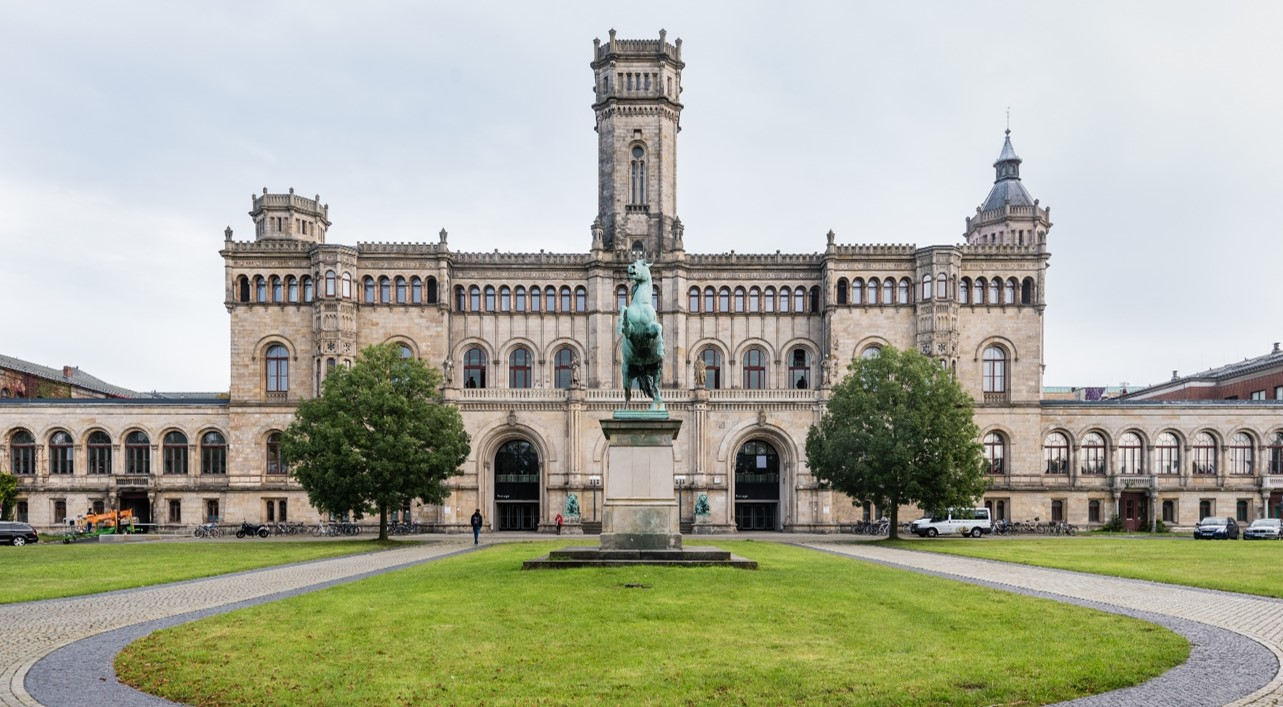
\includegraphics[width=0.65\textwidth]{figures/luh_default_presentation_title_image.jpg}}

% Title page: luhstyle
% \setbeamertemplate{title page}[luhstyle]
% % Add optional title image here
% \addtitlepageimage{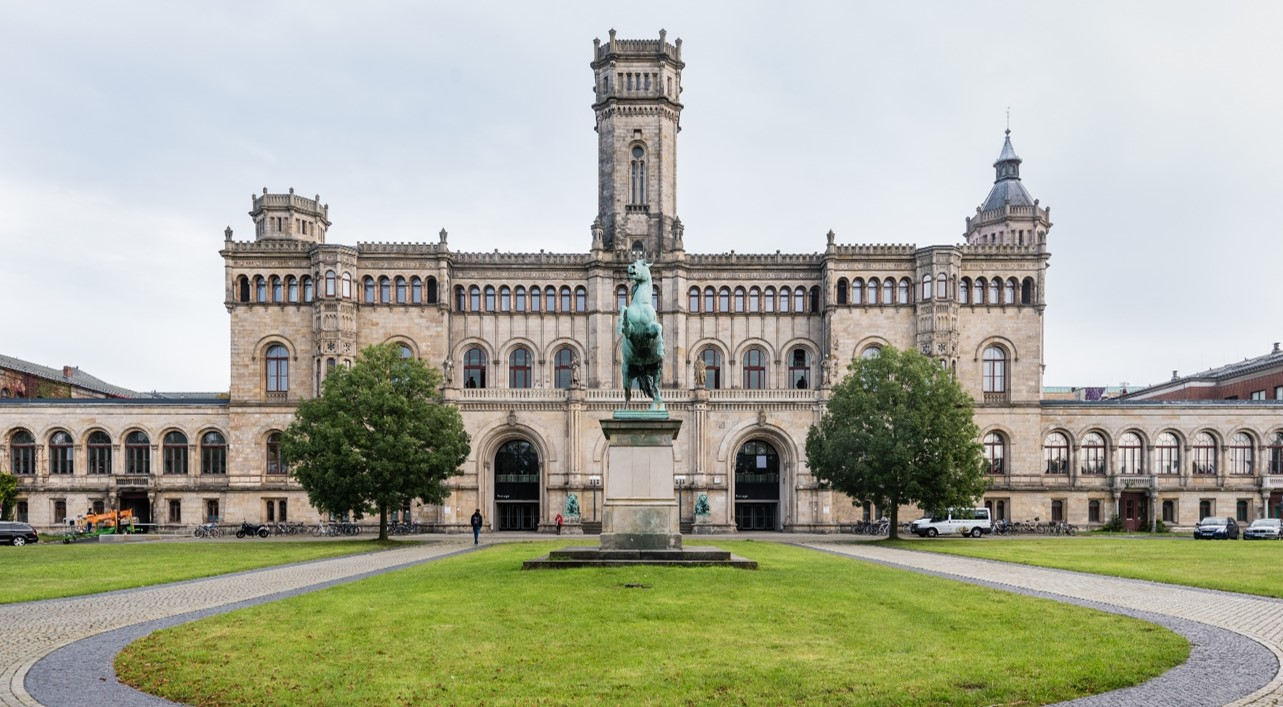
\includegraphics[width=0.75\textwidth]{figures/luh_default_presentation_title_image.jpg}}

\author[Abedjan \& Lindauer]{Ziawasch Abedjan \& Marius Lindauer\\[1em]
	
\includegraphics[height=\logoheight]{../latex_main/figures/luh_logo_rgb_0_80_155.pdf}\qquad
	
\includegraphics[height=\logoheight]{../latex_main/figures/DBIS_Kurzlogo.png}\qquad

\includegraphics[height=\logoheight]{../latex_main/figures/TNT_darkv4}\qquad

\includegraphics[height=\logoheight]{../latex_main/figures/L3S.jpg}	}
\date{Summer Term 2022; \hspace{0.5em} {
\includegraphics[height=1.5em]{../latex_main/figures/Cc-by-nc-sa_icon.svg.png}}; based on \href{https://ds100.org/fa21/}{[DS100]}
}


%%% Custom Packages
%----------------------------------------------------------------------
% Create dummy content
\usepackage{blindtext}

% Adds a frame with the current page layout. Just call \layout inside of a frame.
\usepackage{layout}


%%% Macros
%\renewcommand{\vec}[1]{\mathbf{#1}}
% \usepackage{bm}
%\let\vecb\bm

\title[Introduction]{DS: Bias and Variance}
\subtitle{Data Generation Process}

\graphicspath{ {./figure/} }
%\institute{}


\begin{document}
	
	\maketitle
	\begin{frame}{Data Generation Process}
	    \begin{columns}
	        \begin{column}{.4\textwidth}
	                \begin{figure}
	                    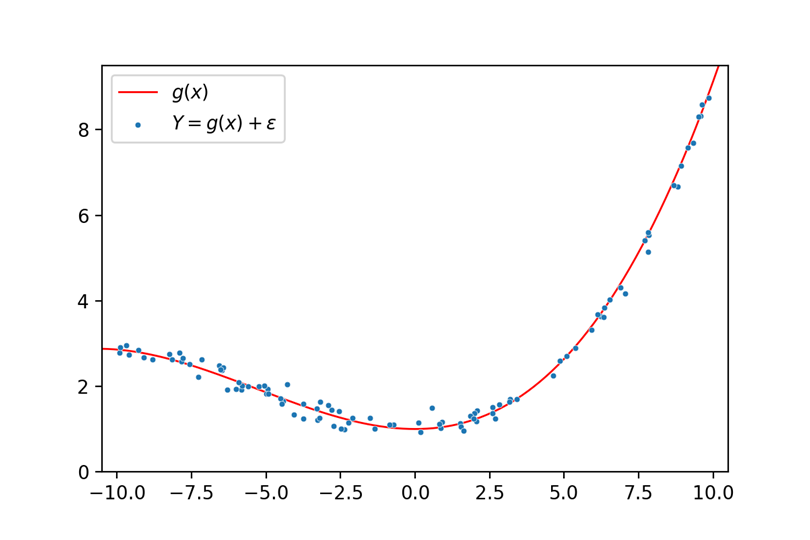
\includegraphics[scale=.5]{Bild1}
	                \end{figure}
	        \end{column}
	        
	        
	         \begin{column}{.4\textwidth}
	            \\ \bigskip
	            \bigskip
	            \bigskip
	                \begin{itemize}
	                    \item Assume true relation g
	                    \item For example: $g(x) = \theta_0 + \theta_1x$
	                    \item For each individual:
	                    \begin{itemize}
	                        \item fixed value of x, so also g(x)
	                        \item random error $\epsilon$
	                        \item Observation is:
	                        \begin{equation*}
	                            Y = g(x) + \epsilon
	                        \end{equation*}
	                    \end{itemize}
	                \end{itemize}
	        \end{column}
	    \end{columns}
	    Errors $\epsilon$ have expectation 0, and are “iid” across individuals

	\end{frame}
	
	
	\begin{frame}{The Data}
	    \begin{columns}
	        \begin{column}{.4\textwidth}
	                \begin{itemize}
	                    \item At each x, truth is g(x)
	                    \item noise is $\epsilon$
	                    \item Observation is $Y = g(x) + \epsilon$
	                \end{itemize}
	                \begin{figure}
	                    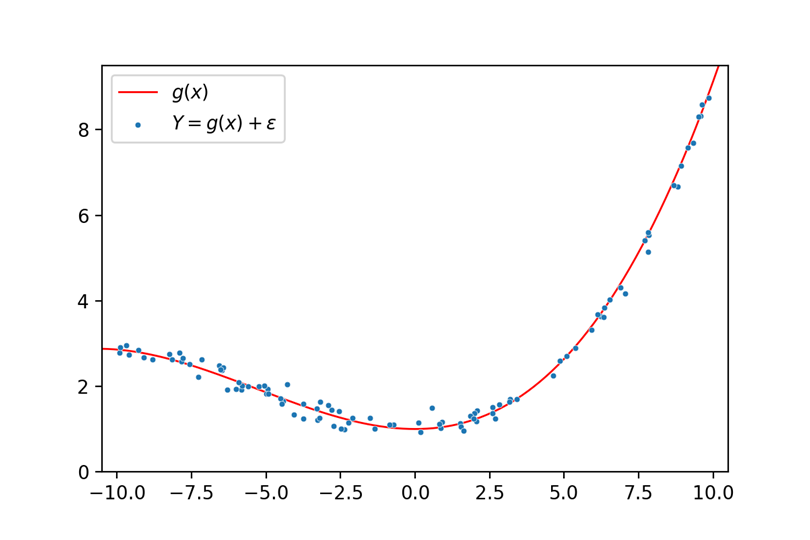
\includegraphics[scale=.4]{Bild1}
	                \end{figure}
	        \end{column}
	        
	        
	         \begin{column}{.4\textwidth}
	         \\ \bigskip
	         \bigskip
	         \bigskip
	         \medskip
	               We only see Y
	                \begin{figure}
	                    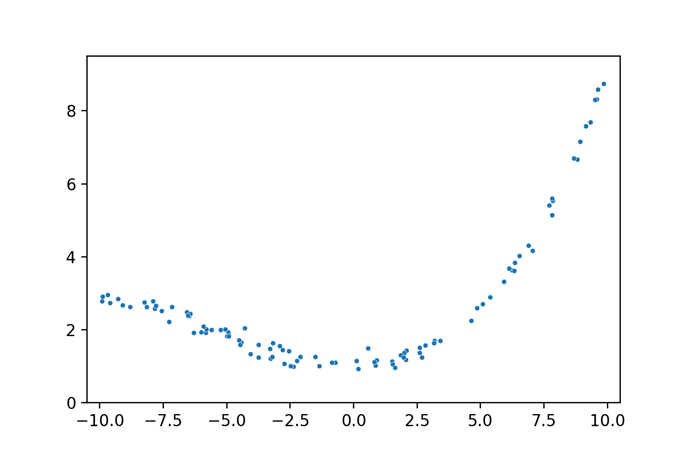
\includegraphics[scale=.45]{Bild2}
	                \end{figure}
	        \end{column}
	    \end{columns}
	\end{frame}
	
	
	\begin{frame}{Our Predictions}
	    \begin{itemize}
	        \item We choose a model and fit it to our data
	        \begin{itemize}
	            \item Choosing a model is codifying our assumption of the form of g(x)
	        \end{itemize}
	        \item The red line is our fitted function—the best possible function given g(x)
	    \end{itemize}
	    \begin{columns}
	        \begin{column}{.4\textwidth}
	                \begin{figure}
	                    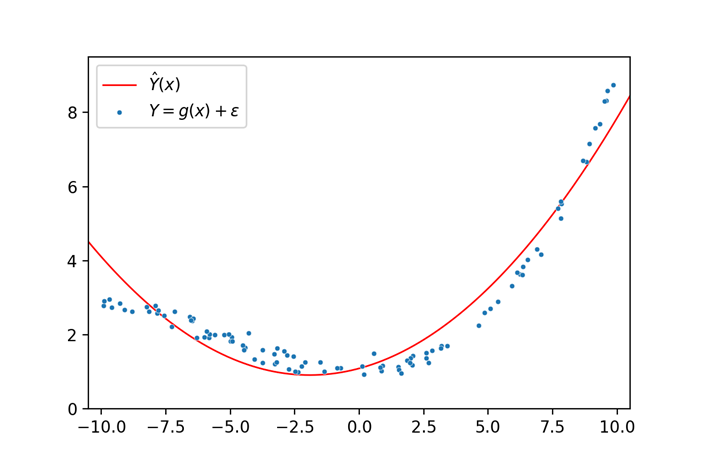
\includegraphics[scale=.5]{Bild3}
	                \end{figure}
	        \end{column}
	        
	        
	         \begin{column}{.4\textwidth}
	         \\ \bigskip
	         \bigskip
	               At every x, our prediction for Y is
	                \begin{itemize}
	                    \item the height of the red line at x
	                    \item Denote this  \hat{Y}(x)
	                \end{itemize}
	        \end{column}
	    \end{columns}
	\end{frame}
	
	
	\begin{frame}{Random Variable}
	    \begin{columns}
	        \begin{column}{.4\textwidth}
	                A random variable is a variable that can takes numerical values with particular probabilities.\\
	                \bigskip
	                Example 1:\\
                    Let X take the value 1 if FDR, 0 if \\
                    Landon\\
                    \bigskip
                    Example 2:\\
                    Let Y be the \# of pips on a roll of a \\
                    6-sided die



	        \end{column}
	        
	        
	        \begin{column}{.4\textwidth}
	            Notation:
	                \begin{itemize}
	                    \item Random variables (RVs) use capital letters
	                    \begin{itemize}
	                        \item X, Y, Z
	                    \end{itemize}
	                    \item A particular value taken by an RV is indicated by a lowercase letter.
	                    \begin{itemize}
	                        \item x, y, z
	                    \end{itemize}
	                    \item The (Probability) Distribution of a discrete RV can be expressed as a table or graphic.
	                    \begin{itemize}
	                        \item P(X = x)
	                    \end{itemize}
	                \end{itemize}
	        \end{column}
	    \end{columns}
	\end{frame}
	
	
	\begin{frame}{Discrete vs. Continuous}
	    \begin{columns}
	        \begin{column}{.4\textwidth}
	               Most random variables we have discussed so far follow discrete distributions.\\

	               RVs following discrete distributions can only take on specific values, and are defined by their Probability Mass Function.\\

	               Example: Binomial Distribution.
                    \begin{figure}
                        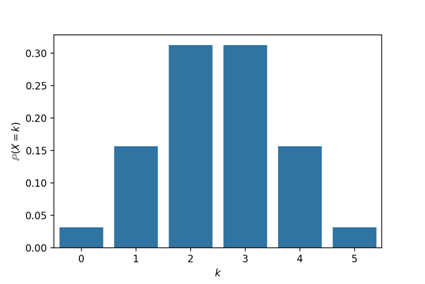
\includegraphics[scale=.5]{Bild4}
                    \end{figure}
	        \end{column}
	        
	        
	        \begin{column}{.4\textwidth}
	            Other random variables, like ε, follow continuous distributions.\\

	               RVs following continuous distributions take on values to arbitrary precision, and are defined by their Probability Density Function.\\
	               Example: Normal Distribution.\\
	               \bigskip
                    \begin{figure}
                        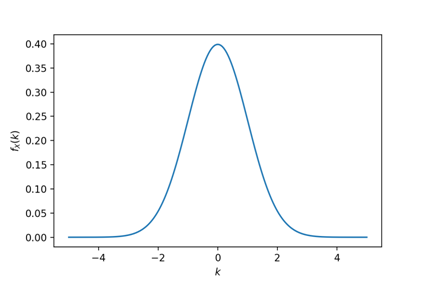
\includegraphics[scale=.5]{Bild5}
                    \end{figure}
	        \end{column}
	    \end{columns}
	\end{frame}
	
	
	\begin{frame}{Expectations}
	    The expectation of a random variable X is the weighted average of the values of X, where the weights are the probabilities of the values.
	    \begin{columns}
	        \begin{column}{.4\textwidth}
                    \begin{figure}
                        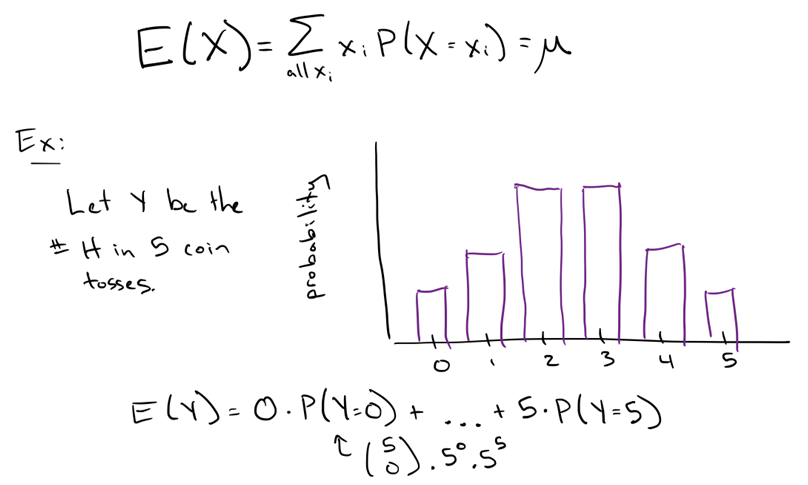
\includegraphics[scale=.5]{Bild6}
                    \end{figure}
	        \end{column}
	        
	        
	        \begin{column}{.4\textwidth}
	            \begin{itemize}
	                \item Expectation is a number, not a random variable
	                \item It is analogous to the average.
	                \begin{itemize}
	                    \item It has the same units as the random variable.
	                    \item It doesn’t need to be a possible value of the random variable.
	                    \item It is the center of gravity of the probability histogram.
	                \end{itemize}
	            \end{itemize}
	        \end{column}
	    \end{columns}
	\end{frame}
	
	
	
	\begin{frame}[c]{Properties of Expectations}
	    Linear transformations\\
	    Let $Z = aX + b;\hspace{5mm} \mathbb{E}(Z) = \mathbb{E}( aX + b) = a\mathbb{E}(X) + \mathbb{E}(b) = a\mathbb{E}(X) + b$\\
	    \bigskip
	    Additivity\\
	    Let $W = X_1 + X_2; \hspace{5mm} \mathbb{E}(W) = \mathbb{E}( X_1 + X_2) =  \mathbb{E}( X_1) + \mathbb{E}(X_2)$\\
	    \bigskip
	    Linearity of Expectation\\
	    Let $V = aX_1 + bX_2;\hspace{5mm} \mathbb{E}(V) = \mathbb{E}( aX_1 + bX_2) = a\mathbb{E}(X_1) + b\mathbb{E}(X_2)  $
	\end{frame}
	
	
	\begin{frame}[c]{Expectation of a Function of a Random Variable}
	    What if we want to calculate E(X2)? Or more generally, E( f(X) )? Does this equal f( E(X) )?\\
	    NO!\\
	    Let’s work through an example with the distribution of one six-sided die roll:
	    \begin{align*}
	        \mathbb{E}(f(x)) &= \sum\limits_kf(k)\mathbb{P}(X=k)\\
	        \mathbb{E}(X^2) &= \sum\limits_kk^2\mathbb{P}(X=k)\\
	        &= 1^2\cdot \frac{1}{6} + 2^2\cdot \frac{1}{6} + 3^2\cdot \frac{1}{6} + 4^2\cdot \frac{1}{6} +  5^2\cdot \frac{1}{6} + 6^2\cdot \frac{1}{6} = \frac{91}{6}\\
	        \mathbb{E}(X^2) &\neq (\mathbb{E}(X))^2 = \left(\frac{7}{2}\right)^2 = \frac{49}{4}
	    \end{align*}
	\end{frame}
	
	
	\begin{frame}[c]{Estimators and Bias}
	    Recall that parameters represent the truth, and we estimate these parameters with statistics\\
	    Take the function: $g(x) = \theta_0 + \theta_1x$\\
	   $\theta_0$ and $\theta_1$ are parameters. We estimate them with:
	    \begin{align*}
	       \hat{\theta}_1 = r\frac{\sigma_y}{\sigma_x}\hspace{5mm} \hat{\theta}_0 = \overline{y} - \hat{\theta}_1\overline{x}
	    \end{align*}
	    Recall that statistical bias is the expected difference between your estimate and the truth.
        \begin{align*}
            \mathbb{E}(\hat{\theta} - \theta) = \mathbb{E}(\hat{\theta}) - \theta
        \end{align*}
        Remember, $\hat{\theta}$	is random! It is random because the dataset you sample is random.\\
        (We can prove that the above estimates for $\theta_0$ and $\theta_1$ are unbiased, but we will not do so here.)

	\end{frame}
	
	
	\begin{frame}[c]{Summary}
	   \begin{itemize}
	       \item Random variables are functions of our sample.
	       \item The expectation of a random variable is the weighted average of its possible values, weighted by the probabilities of those values.
	       \begin{itemize}
	           \item Expectation behaves nicely with linear transformations of random variables.
	           \item Expectation is also additive.
	           \item We can calculate the expectation of a function of a random variable.
	       \end{itemize}
	       \item The optimal weights in our linear models are estimates of the true parameters.
	   \end{itemize}
	\end{frame}
	
	\begin{frame}{Definition of variance}
	    \begin{itemize}
	        \item Variance is the expected squared deviation from the expectation of X.
	        \item It is defined as follows:
	        \begin{equation*}
	            \mathbb{Var}(X) = \mathbb{E}((X - \mathbb{E}(X))^2)
	        \end{equation*}
	        \item The units of the variance are the square of the units of X
	        \item To get back to the right scale, we look at the standard deviation of X:
	        \begin{equation*}
	            \mathbb{SD}(X)  = \sqrt{\mathbb{Var}(X)}  =\sqrt{\mathbb{E}((X - \mathbb{E}(X))^2)}
	        \end{equation*}
	        \item Both standard deviation and variance must be non-negative.
	    \end{itemize}
	\end{frame}
	
	
	\begin{frame}[c]{Interpretation of variance}
	    \begin{itemize}
	        \item The main use of variance is to quantify chance error.
	        \begin{itemize}
	            \item How far away from the expectation can X be, just by chance?
	        \end{itemize}
	        \item By Chebyshev’s inequality from Data 8:
	        \begin{itemize}
	            \item No matter what the shape of the distribution of X is,
	            \item The vast majority of the probability lies in the interval “expectation plus or minus a few SDs”.
	            \item Specifically, if   $\mu$  = E[X] and    $\sigma$   = SD[X], then $P(|X - \mu| \leq \frac{1}{k^2})$.   
	            \item We will not be using this formula in this class; it’s just here to remind you of it.
	            \begin{itemize}
	                \item Here’s a link to a discussion in the Data 8 book about this.
	            \end{itemize}
	        \end{itemize}
	    \end{itemize}
	\end{frame}
	
	
	\begin{frame}[c]{An alternative calculation}
	    There’s a more convenient form of variance for use in calculations.
	    \begin{equation*}
	        \mathbb{Var}(X) = \mathbb{E}(X^2) - (\mathbb{E}(X))^2
	    \end{equation*}
	    To derive this, we make repeated use of the linearity of expectation.
	    \begin{align*}
	        \mathbb{Var}(X) &= \mathbb{E}((X-\mathbb{E}(X))^2)\\
	        &=  \mathbb{E}(X^2-2X\mathbb{E}(X) + (\mathbb{E}(X)^2))\\
	        &= \mathbb{E}(X^2) - 2\mathbb{E}(X)\mathbb{E}(X) + (\mathbb{E}(X))^2\\
	        &= \mathbb{E}(X^2) - (\mathbb{E}(X))^2
	    \end{align*}
	\end{frame}
	
	
	
	\begin{frame}[c]{An alternative calculation}
	    \begin{equation*}
	        \mathbb{Var}(X) = \mathbb{E}(X^2) - (\mathbb{E}(X))^2
	    \end{equation*}
	    For example, to compute the variance of one roll of a die, we can find
	    \begin{equation*}
	        \mathbb{Var}(X) = (1^2+2^2+3^2+4^2+5^2+6^2)\cdot \frac{1}{6}-(3.5)^2 = 2.92
	    \end{equation*}
	    
	    \begin{itemize}
	        \item This formulation also makes clear that if X is centered, i.e. $\mathbb{E}$(X) = 0, then $\mathbb{Var}$(X) = $\mathbb{E}$($X^2$).
	        \item Since $\mathbb{Var}$(X) is non-negative, this property also shows us that                   $\mathbb{E}(X^2) \geq (\mathbb{E}(X))^2$.      Equality is if and only if X is a constant.
	        \item If you know the expectation and variance of a random variable, you can easily determine the expectation of its square:   $\mathbb{E}(X^2) = \mathbb{Var}(X) + (\mathbb{E}(X))^2$. 
	    \end{itemize}
	\end{frame}
	
	
	\begin{frame}[c]{Linear transformations}
	    We know that  $\mathbb{E}(aX + b) = a\mathbb{E}(X) + b$. In order to compute Var(aX + b), consider:\\
	    \begin{columns}
	        \begin{column}{.4\textwidth}
	                A shift by b units does not affect spread:
	                \begin{figure}
	                    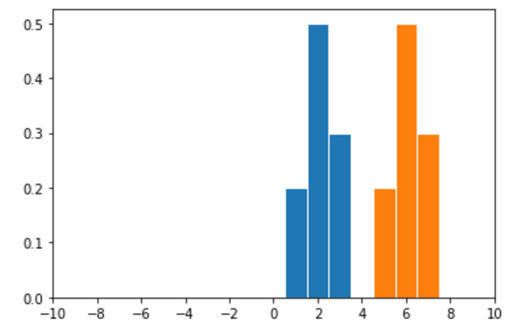
\includegraphics[scale=.5]{Bild7}
	                \end{figure}
	                Here, the distribution of X is in blue, and the distribution of X+4 is in orange.
	        \end{column}
	        
	        
	        \begin{column}{.4\textwidth}
	                But scaling by a units does affect spread:
	                \begin{figure}
	                    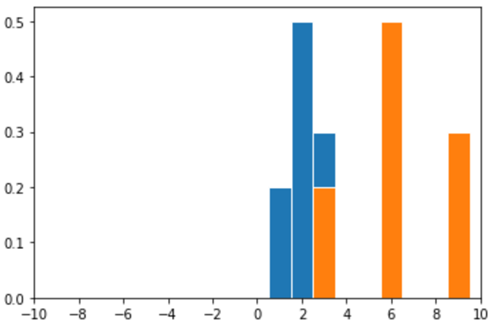
\includegraphics[scale=.35]{Bild8}
	                \end{figure}
	                The distribution of X is in blue, and the distribution of 3X is in orange. 
	        \end{column}
	    \end{columns}
	\end{frame}
	
	
	\begin{frame}[c]{Linear transformations}
	   We know that       $\mathbb{E}(aX + b) = a\mathbb{E}(X) + b$. \\                  In order to compute $\mathbb{Var}$(aX + b), consider:
	    \begin{itemize}
	        \item A shift by b units does not affect spread. Thus, $\mathbb{Var}$(aX + b) = $\mathbb{Var}$(aX).
	        \item The multiplication by a does affect spread!
	    \end{itemize}
	    Then,
	    \begin{align*}
	        \mathbb{Var}(aX + b) = \mathbb{Var}(aX) &= \mathbb{E}((aX)^2) - (\mathbb{E}(aX))^2\\
	        &= \mathbb{E}(a^2X^2) - (a\mathbb{E}(X))^2\\
	        &= a^2(\mathbb{E}(X^2) - (\mathbb{E}(X))^2)\\
	        &= a^2\mathbb{Var}(X)
	    \end{align*}
	    In summary:
	    \begin{align*}
	        \mathbb{Var}(aX + b) &= a^2\mathbb{Var}(X)\\
	        \mathbb{SD}(aX + b) &= |a|\mathbb{SD}(X)
	    \end{align*}
	\end{frame}
	
	
	\begin{frame}[c]{Standardization of random variables}
	   X in standard units is the random variable $X_{su} = \frac{X- \mathbb{E}(X)}{\mathbb{SD}(X)}$
	   \begin{itemize}
	       \item $X_{su}$ measures X on the scale “number of SDs from expectation.”
	       \item It is a linear transformation of X. By the linear transformation rules for expectation and variance:
	       \begin{equation*}
	           \mathbb{E}(X_{su})  = 0, \hspace{5mm} \mathbb{SD}(X_{su}) = 1
	       \end{equation*}
	       \item Since $X_{su}$ is centered (has expectation 0):
	       \begin{equation*}
	           \mathbb{E}(X^2_{su}) = \mathbb{Var}(X_{su}) = 1
	       \end{equation*}
	       You should prove these facts yourself.
	   \end{itemize}
	\end{frame}
	
	\begin{frame}[c]{Covariance}
	   The covariance of two random variables is their expected product of deviations.
	   \begin{equation*}
	       \mathbb{Cov}(X,Y) = \mathbb{E}((X-\mathbb{E}(X))(Y-\mathbb{E}(Y)))
	   \end{equation*}
	   \begin{itemize}
	       \item It is a generalization of variance. Note:   $\mathbb{Cov}(X,X) = \mathbb{Var}(X)$.   
	       \item Using the linearity of expectation and some algebra, you can show the following equality, which is a generalization of the alternative calculation for variance:
	       \begin{equation*}
	           \mathbb{Cov}(X,Y) = \mathbb{E}(XY) - \mathbb{E}(X)\mathbb{E}(Y)
	       \end{equation*}
	       \item To see whether variance is ever additive, we need to look at covariance differently.
	   \end{itemize}
	\end{frame}
	
	\begin{frame}[c]{Correlation}
	   The units of the covariance are hard to interpret (e.g. “inch pounds”). In order to get rid of the units, we can scale it:
	   \begin{align*}
	       \frac{\mathbb{Cov}(X,Y)}{\mathbb{SD}(X)\mathbb{SD}(Y)}  &= \frac{ \mathbb{E}((X-\mathbb{E}(X))(Y-\mathbb{E}(Y)))}{\mathbb{SD}(X)\mathbb{SD}(Y)}\\
	       &= \mathbb{E}\left( \frac{X-\mathbb{E}(X)}{\mathbb{SD}(X)} \cdot \frac{Y-\mathbb{E}(Y)}{\mathbb{SD}(Y)}\right)\\
	       &= \mathbb{E}(X_{su}Y_{su})\\
	       &= r(X,Y)
	   \end{align*}
	   Recall from Data 8: correlation is the average product in standard units. This is the random variable equivalent of that!

	   Correlation is covariance scaled by the two SDs.
	\end{frame}
	
	
		\begin{frame}{A Constant Model}
	    Let’s say you want to estimate how often a coin lands on heads when flipped.
	    \begin{itemize}
	        \item The result of a coin flip follows a Bernoulli(p) distribution, and you want to estimate p.
	        \item You do not collect any data, but instead you are given a choice between two models.
	        \item Suppose you are also told that p = .5.
	    \end{itemize}
	    Which of the following is the better model?\\
	    \bigskip
	    Model A: Select a random number between 0 and 1. This is your estimate of p. This is equivalent to running np.random.random()in Python.\\
	    \bigskip
	    Model B: Select .75 as your estimate of p.
	\end{frame}
	
	
	\begin{frame}{A Constant Model}
	   How do we define “better”?\\
	   \bigskip
	    We can calculate the expected MSE of each model. This is called the “model risk,” a term which we will formalize later on. The lower the risk, the better.\\
	    \bigskip
	    Model A: On average, we will select .5 as our estimate, so we expect 0 error. But, as we are only selecting one number, there is a chance we select a number really far away from .5.\\
	    \bigskip
	    Model B: With this model, we will never be exactly correct. But, we know there is zero chance of a really terrible prediction.
	\end{frame}
	
	
	\begin{frame}[c]{The Bias-Variance Tradeoff}
	   When building models, we generally face a tradeoff between bias and variance.
	   \begin{itemize}
	       \item Lower bias means that our model will predict closer to the truth, on average.
	       \item Lower variance means that our model will not change too much given the sample.
	   \end{itemize}
	   \bigskip
	   We want low bias and low variance, but oftentimes, when one decreases, the other increases.\\
	   Model A has zero bias, but lots of variance. Model B has zero variance, but lots of bias.\\
	   \bigskip
	   So which is better? The answer will be revealed later in the lecture.
	\end{frame}
	
	
	\begin{frame}[c]{Three Sources of Error in Our Predictions}
	   Irreducible error: Recall the data generating process: $Y = g(x) + \epsilon$
	   \begin{equation*}
	       \mathbb{Var}(\epsilon) = \sigma^2 \hspace{5mm} \mathbb{Var}(Y) = \mathbb{Var}(g(x) + \epsilon) = \mathbb{Var}(\epsilon) = \sigma^2
	   \end{equation*}
	   There will be chance error in our predictions due to the natural randomness of the world.\\
	   \bigskip
	   Model variance: Our fitted model is based on a random sample.\\
        The sample could have come out differently, then the fitted model would have been different.\\
        \bigskip
        Model bias: This is the difference between the expected predictions, and the true g(x).\\
        Our model may be too limited to find the correct g(x), for example if we pick a quadratic model to fit to cubic data.

	\end{frame}
	
	
	\begin{frame}[c]{Simulation}
	  \begin{columns}
	      \begin{column}{.6\textwidth}
	           \begin{figure}
	               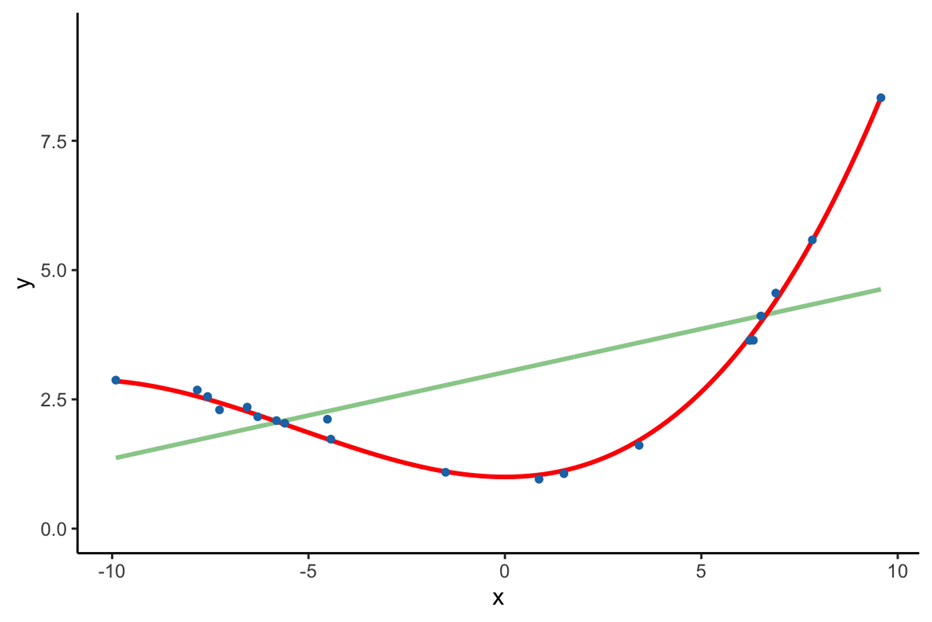
\includegraphics[scale=.5]{Bild9}
	           \end{figure} 
	      \end{column}
	      
	      \begin{column}{.4\textwidth}
	      \\
	      \bigskip
	      \bigskip
	      \bigskip
	            Let’s simulate the sampling and modeling process for a strictly linear model.\\
	            $g(x) = \theta_0 + \theta_1x$
	      \end{column}
	  \end{columns}
	\end{frame}
	
	\begin{frame}[c]{Simulation}
	  \begin{columns}
	      \begin{column}{.6\textwidth}
	           \begin{figure}
	               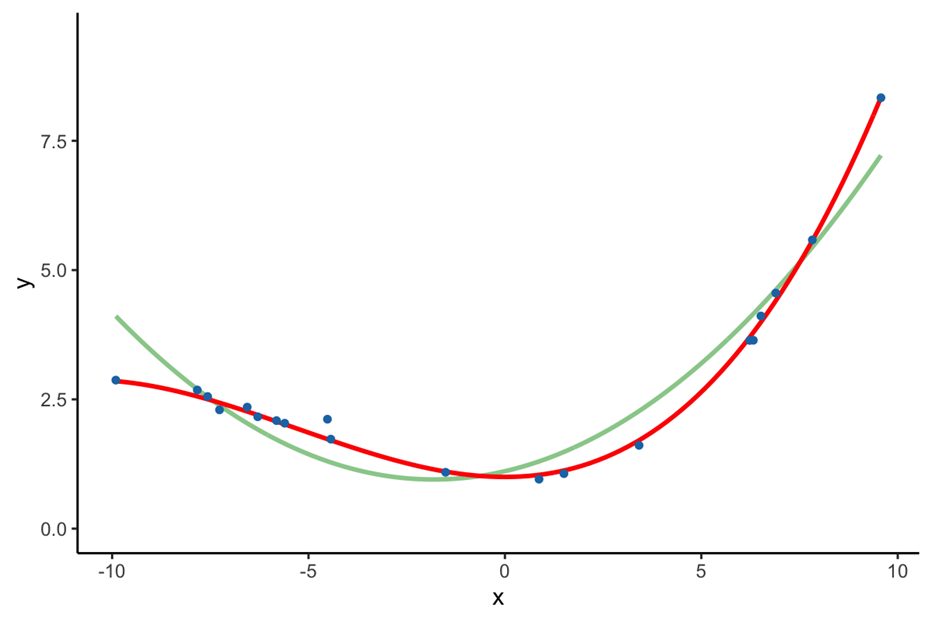
\includegraphics[scale=.5]{Bild10}
	           \end{figure} 
	      \end{column}
	      
	      \begin{column}{.4\textwidth}
	      \\
	      \bigskip
	      \bigskip
	      \bigskip
	            Let’s simulate the sampling and modeling process for a quadratic model.\\
	            $g(x) = \theta_0 + \theta_1x + \theta_2x^2$
	      \end{column}
	  \end{columns}
	\end{frame}
	
	
	\begin{frame}[c]{Simulation}
	  \begin{columns}
	      \begin{column}{.6\textwidth}
	           \begin{figure}
	               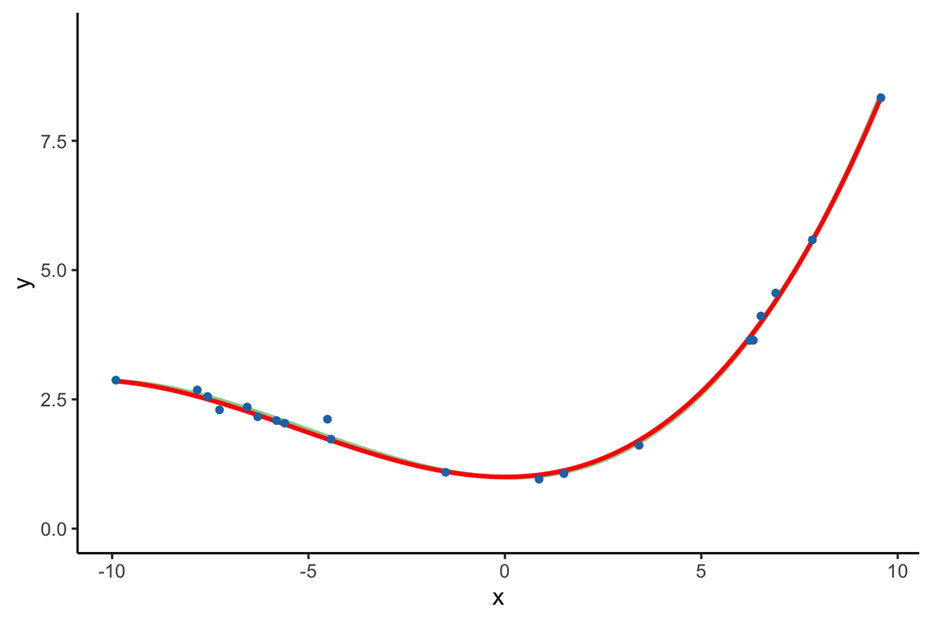
\includegraphics[scale=.5]{Bild11}
	           \end{figure} 
	      \end{column}
	      
	      \begin{column}{.4\textwidth}
	      \\
	      \bigskip
	      \bigskip
	      \bigskip
	            Let’s simulate the sampling and modeling process for a cubic model.\\
	            $g(x) = \theta_0 + \theta_1x + \theta_2x^2 + \theta_3x^3$
	      \end{column}
	  \end{columns}
	\end{frame}
	
	
	
	\begin{frame}[c]{Simulation}
	  \begin{columns}
	      \begin{column}{.6\textwidth}
	           \begin{figure}
	               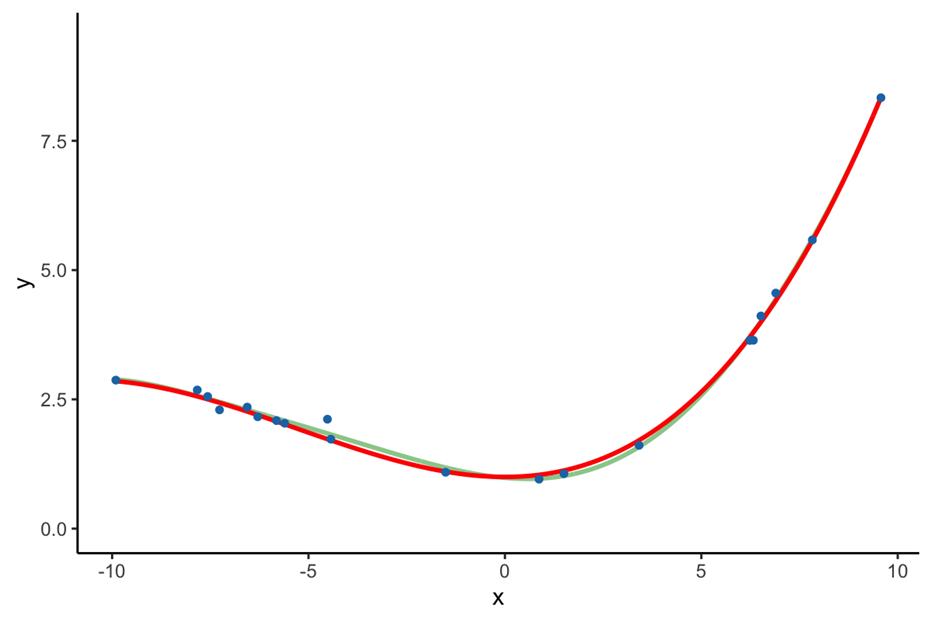
\includegraphics[scale=.5]{Bild12}
	           \end{figure} 
	      \end{column}
	      
	      \begin{column}{.4\textwidth}
	      \\
	      \bigskip
	      \bigskip
	      \bigskip
	           Let’s simulate the sampling and modeling process for a septic model.\\
	            $g(x) = \theta_0 + \sum\limits_{i=1}^7 \theta_ix^i$
	      \end{column}
	  \end{columns}
	\end{frame}
	
	\begin{frame}[c]{Diagram}
	  \begin{columns}
	     
	      
	      \begin{column}{.4\textwidth}
	      \\
	      \bigskip
	      \bigskip
	      \bigskip
	          Red line (fixed): g(X)\\
	          Green line $\mathbb{E}(\hat{Y}(x))$
	          \begin{itemize}
	              \item This is fixed, given our model.
	          \end{itemize}
	          Gray lines: Possible $\hat{Y}(x)$\\
	          Blue points: Y = g(x) + $\epsilon$
	      \end{column}
	      
	      
	       \begin{column}{.6\textwidth}
	           \begin{figure}
	               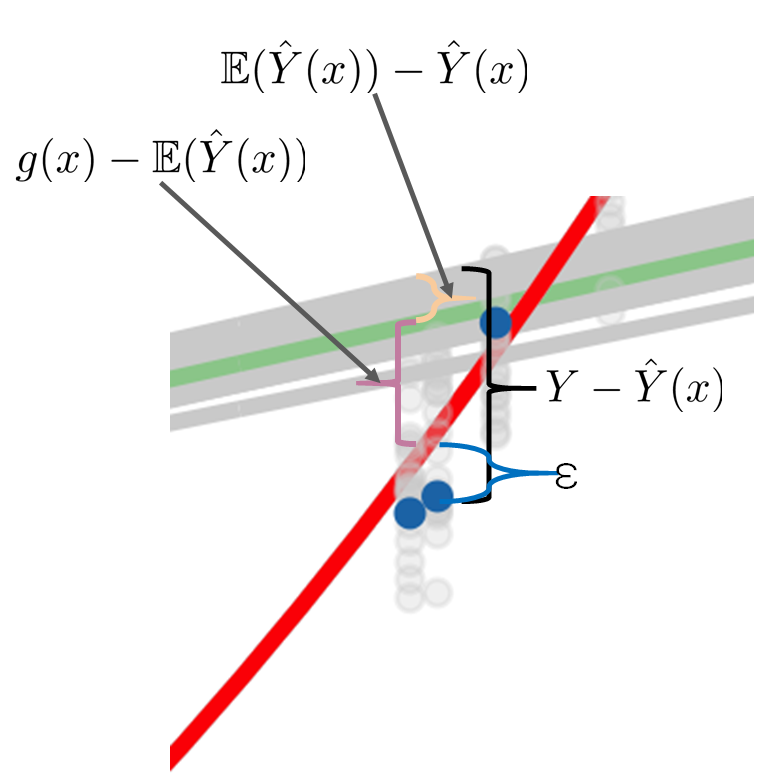
\includegraphics[scale=.3]{Bild13}
	           \end{figure} 
	      \end{column}
	  \end{columns}
	\end{frame}
	
		\begin{frame}{Model Risk}
	    For a new individual at (x, Y):
	    \begin{itemize}
	        \item Expected mean squared error of prediction:
	        \begin{equation*}
	            \text{model risk} = \mathbb{E}((Y-\hat{Y}(x))^2)
	        \end{equation*}
	    \end{itemize}
	    The expectation is taken over all possible samples that we could have collected.
	    \begin{itemize}
	        \item Remember, each new sample would generate a different $\hat{Y}(x)$
	        \item Also, for some fixed x, Y can be different due to the random error $\epsilon$
	    \end{itemize}
	\end{frame}
	
	
	\begin{frame}[c]{Decomposition of Error and Risk}
	    The model risk can be decomposed into three pieces:
	    \begin{align*}
	        \mathbb{E}((Y-\hat{Y}(x))^2) &= \mathbb{E}(\epsilon^2)\\
	        &+ (g(x) - \mathbb{E}(\hat{Y}(x)))^2\\
	        &+ \mathbb{E}((\mathbb{E}(\hat{Y}(x))-\hat{Y}(x))^2)
	    \end{align*}
	    \begin{equation*}
	        \text{model risk} = \sigma^2 + (\text{model bias})^2 + \text{model variance}
	    \end{equation*}
	    See the video for the derivation!
	\end{frame}
	
	
	\begin{frame}[c]{Observation Variance}
	    \begin{equation*}
	        \mathbb{Var}(Y) = \mathbb{Var}(g(x) + \epsilon) = \mathbb{Var}(\epsilon) = \sigma^2
	    \end{equation*}
	    Some reasons:
	    \begin{itemize}
	        \item Measurement error
	        \item Missing information acting like noise
	    \end{itemize}
	    \bigskip
	    Some remedies:
	    \begin{itemize}
	        \item Could try to get more precise measurements.
	        \item Often this is beyond the control of the data scientist.
	    \end{itemize}
	\end{frame}
	
	\begin{frame}[c]{Model Variance}
	    \begin{equation*}
	        \text{model variance} = \mathbb{Var}(\hat{Y}(x)) = \mathbb{E}((\hat{Y}(x) - \mathbb{E}(\hat{Y}(x)))^2)
	    \end{equation*}
	    Main reason:
	    \begin{itemize}
	        \item Overfitting: small differences in random samples lead to large differences in the fitted model
	    \end{itemize}
	    \bigskip
	    Some remedies:
	    \begin{itemize}
	        \item Reduce model complexity
	        \item Don’t fit the noise
	    \end{itemize}
	\end{frame}
	
	
	\begin{frame}[c]{Model Bias}
	    \begin{equation*}
	        \text{model bias} = \mathbb{E}(\hat{Y}(x)) - g(x)
	    \end{equation*}
	    Some reasons:
	    \begin{itemize}
	        \item Underfitting
	        \item Lack of domain knowledge
	    \end{itemize}
	    \bigskip
	    Remedies:
	    \begin{itemize}
	        \item Increase model complexity (but don’t overfit)
	        \item Consult domain experts to see which models make sense
	    \end{itemize}
	\end{frame}
	
	
	\begin{frame}[c]{A Constant Model}
	    So which model is better? Model A or Model B?\\
	    \bigskip
	    Model A: Select a random number between 0 and 1. This is your estimate of p. This is equivalent to running np.random.random()in Python.\\
        Model B: Select .75 as your estimate of p.\\
        \bigskip
        We can calculate the model risks directly. Note that the observation variance is 0.
        \begin{columns}
            \begin{column}{.4\textwidth}
                  Model A:\\
                  \bigskip
                  Model Bias = .5 - .5 = 0\\
                  Model Variance = (1 - 0)$^2$ / 12 = 1/12\\
                  \bigskip
                  Risk = 0$^2$ + 1/12 = 1/12
            \end{column}
            
            
            \begin{column}{.4\textwidth}
                   Model B:\\
                  \bigskip
                  Model Bias = .75 - .5 = .25\\
                  Model Variance = 0\\

                  \bigskip
                  Risk = .25$^2$ + 0 = 1/16
 
            \end{column}
        \end{columns}

	\end{frame}
	
	
	\begin{frame}{Introduction to Overfitting}
	    In the previous lectures, our goal has been to minimize a loss function (MSE)
	    \begin{itemize}
	        \item We do this by collecting more features, or through feature engineering
	    \end{itemize}
	    \bigskip
	    However, we only ever evaluated our model on the data on which it was trained
	    \begin{itemize}
	        \item The whole point in building a model is to learn something about the world
	        \item Why do we care about finding a   $\hat{Y}$   if we already know   Y  ?
	    \end{itemize}
	    \bigskip
	    We care about how well our model performs on new data, for which we want to predict Y\\
	    \bigskip
	    To the demo!
	\end{frame}
	
	
	
		\begin{frame}[c]{Modeling Goals}
	    \begin{itemize}
	        \item Try to minimize all three of observation variance, model bias, and model variance.
	    \end{itemize}
	    But
	    \begin{itemize}
	        \item Observation variance is often out of our control
	        \item Reducing complexity to reduce model variance can increase bias
	        \item Increasing model complexity to reduce bias can increase model variance
	        \item Domain knowledge matters: the right model structure!
	    \end{itemize}
	\end{frame}
	
	
	\begin{frame}{Bias Variance Plot}
	    \centering
	    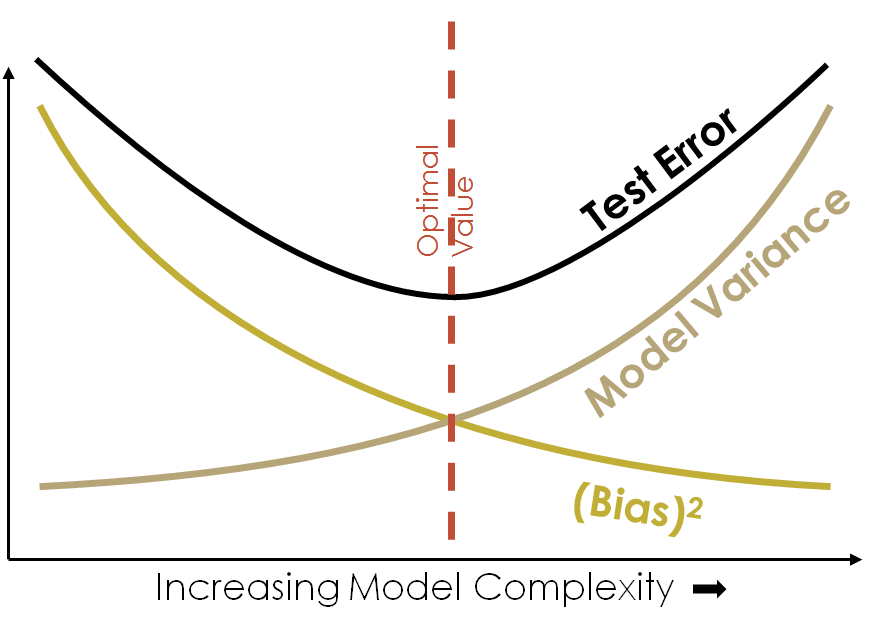
\includegraphics[scale=.4]{Bild14}
	\end{frame}
	
	\begin{frame}{The right model structure matters!}
	    \begin{columns}
	        \begin{column}{.5\textwidth}
	                \begin{figure}
	                    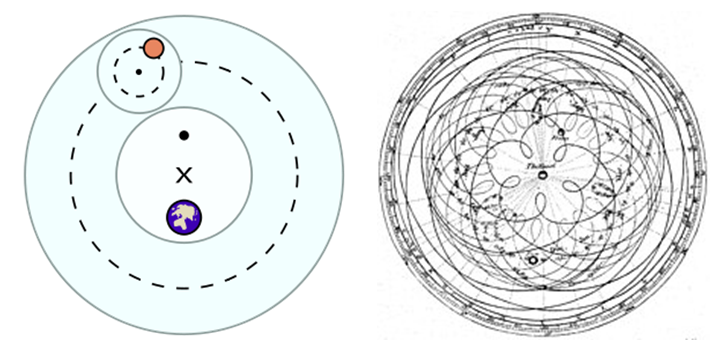
\includegraphics[scale=.35]{Bild15}
	                \end{figure}
	                Ptolemaic Astronomy, a geocentric model based on circular orbits (epicycles and deferents).\\
	                \bigskip
	                High accuracy but very high model complexity.
	        \end{column}
	        
	        
	        \begin{column}{.5\textwidth}
	                \begin{figure}
	                    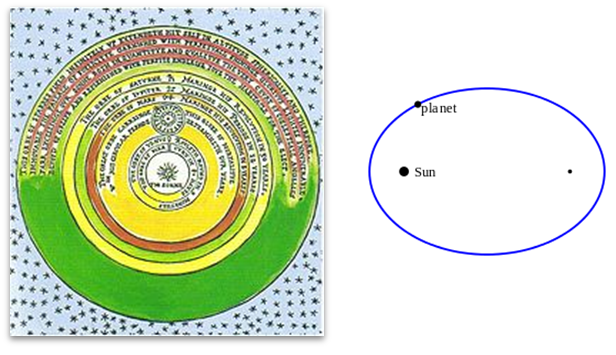
\includegraphics[scale=.35]{Bild16}
	                \end{figure}
	                Copernicus and Kepler: a heliocentric model with elliptical orbits.\\
	                \bigskip
	                Small model complexity yet high accuracy.

	        \end{column}
	    \end{columns}
	\end{frame}
\end{document}